\chapter{CONTRATOS REST COM DESIGN-BY-CONTRACT}


\section{PROPOSTA: SERVIÇOS COM DESIGN-BY-CONTRACT}
\label{PropostaServicoDbC}
\vspace{-6mm}

Os benefícios esperados pela adoção da arquitetura orientada a serviços
somente serão auferidos com a concepção adequada de cada serviço. 
Por essa razão, é necessário planejar o projeto dos serviços criteriosamente
antes de lançar mão do desenvolvimento, com preocupação especial em garantir
um nível aceitável de estabilidade aos consumidores de cada serviço.
Nessa etapa do projeto de desenho da solução, a especificação do contrato do
serviço (Web API) exerce uma função fundamental. 

Na sociedade civil, contratos são meios de se formalizar acordo entre partes a
fim de definir os direitos e deveres de cada parte e buscar atingir o
objetivo esperado dentro de determinadas regras. Cada parte espera que as outras
cumpram com suas obrigações.
Por outro lado, sabe-se que o descumprimeto das obrigações costuma implicar de
penalizações até o desfazimento do contrato. 

Contratos entre serviços Web seguem em uma linha análoga. O desenho das
capacidades (operações) e dos dados das mensagens correspondem aos
termos do contrato no sentido do que o consumidor deve esperar do serviço
provedor. Porém identificou-se, após ampla pesquisa realizada sobre o tema, que
as linguagens disponíves para especificação de contratos atingem apenas esse
nível de garantias. No contexto de webservices em REST, conforme descrito na
seção \ref{secaoREST}, há ainda a ausência de padrão para especificação
contratos.

A proposta deste trabalho é extender os níveis de garantias, de modo a promover
um patamar adicional com obrigações mutuas entre os serviços (consumidor e
provedor). Isso se dá para adoção do conceito de \designbycontract{} (debatido
na seção \ref{Design-by-Contract}) em que a execução da
capacidade do serviço garantirá a execução, desde que satisfeitas as condições
prévias. As próximas subseções detalham o modo de operação dos serviços com as
construções de \designbycontract{}.

\vspace{-6mm}

\subsection{Modelo de operação}
\vspace{-6mm}

As garantias para execução dos serviços são estabelecidas em duas etapas: pré e
póscondições. Nas precondições o provedor do serviço estabelece os requisitos
para que o serviço possa ser executado pelo cliente. A etapa de pós-condições
tem o papel de validar se a mensagem de retorno do serviço possui os resultados
esperados.

O diagrama da Figura \ref{FigServiceDbC} descreve como ocorre a operação das
pré e pós-condições. O processo se inicia com a chamada à capacidade do serviço e a
identificação da existência de uma precondição. Caso tenham sido estabelecidas 
precondições, essas são avaliadas. Caso alguma delas não tenham sido
satisfeitas, o serviço principal não é processado e o provedor do serviço
retornar o código de falha definido no contrato correspondente.


\begin{figure}[!htb]
\centering
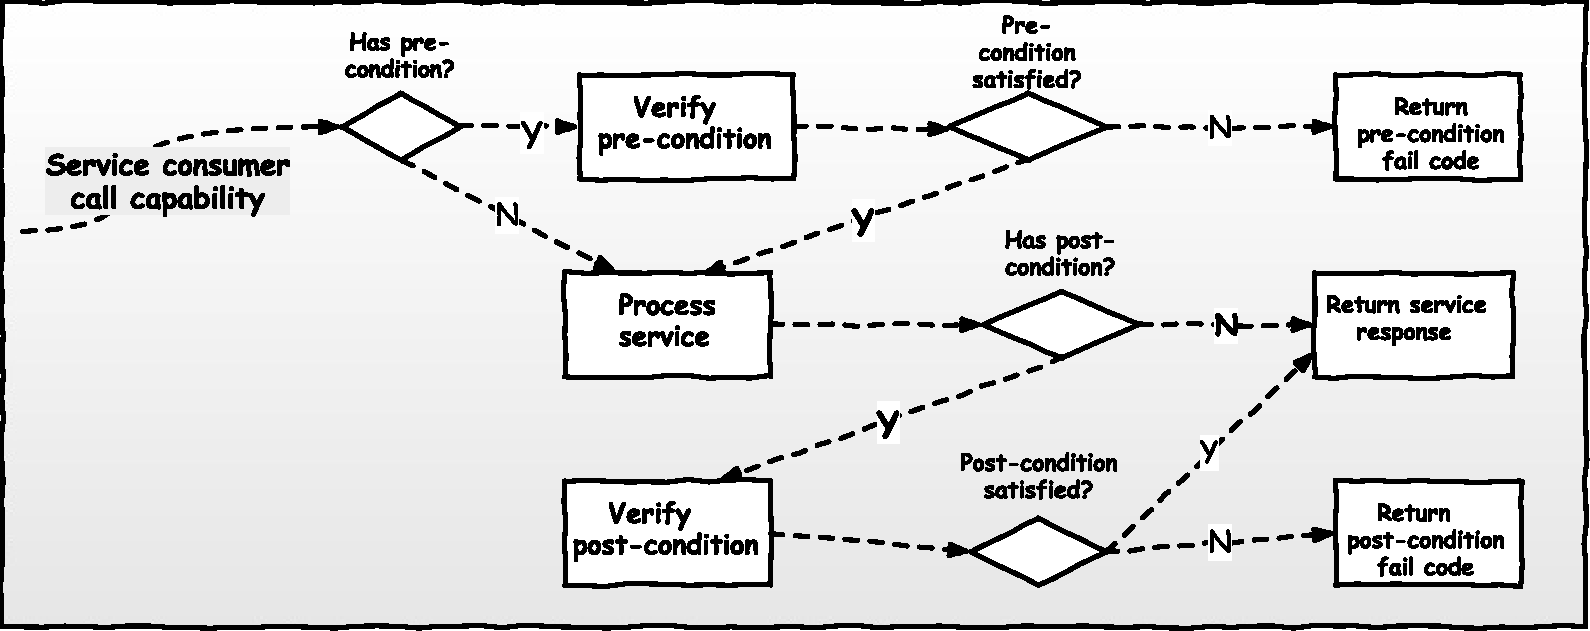
\includegraphics[width=140mm,trim = 0mm 0mm 0mm
0mm,clip]{img/FluxoDbcCondicoes.pdf}
\caption{Digrama de atividades com verificação de pré e pós condições}
\label{FigServiceDbC}
\end{figure}

Caso tenham sido definidas pós-condições, essas são acionadas após o
processamento da capacidade, porém antes do retorno ao consumidor do serviço.
Assim, conforme Figura \ref{FigServiceDbC}, visando não entregar ao cliente uma
mensagem ou situação incoerente, as pós-condições são validadas. Caso todas as
pós-condições tenham sido satisfeitas, a mensagem de retorno é encaminhada ao
cliente. Caso contrário, será retornado o código de falha definido para a
pós-condição violada.

\subsubsection{Observação sobre invariantes}
\vspace{-6mm}

Em \designbycontract{}, além dos conceitos de pré e pós-condições,
há também a ideia de invariantes\cite{meyer1997object}. Quando aplicadas a uma classe na
orientação a objetos, as invariantes estabelecem restrições sobre o estado
armazenado nos objetos instanciados dessa classe. No contexto de orientação a
serviços, tem-se por princípio a ausência de estados dos serviços, descrito na
seção \ref{PrincipiosSOA}. Por essa razão, no estudo sobre a incorporação de
\designbycontract{} em contratos de serviços, as invariantes não foram
consideradas.


\subsection{Verificação das precondições}
\vspace{-6mm}

As precondições podem ser do tipo baseado nos parâmetros da requisição ou do
tipo baseado na chamada a outro serviço. Denomina-se, no contexto desta
dissertação, de básica a precondição baseada apenas nos parâmetros da
requisição (atributos da chamada ao serviço). Essa validação é direta,
comparando os valores passados com os valores admitidos. 

No caso das precondições baseadas em serviços, é realizada chamada a outro
serviço para verificar se uma determinada condição é satisfeita. Este modo de
funcionamento, que se assemelha a uma composição de serviço, é mais versátil, pois permite
validações de condições complexas sem que a lógica associada seja conhecida pelo
cliente. Assim, os contratos que estabelecem esse tipo de
precondição se mantem simples.

A Figura \ref{FigServicePrecondition} detalha as etapas de verificação de cada
precondição. Nota-se que a saída para as situações de desatendimento às
precondições, independentemente do tipo, é o mesmo. O objetivo desta abordagem
é simplificar o tratametno de exceção no consumidor.

\begin{figure}[!htb]
\centering
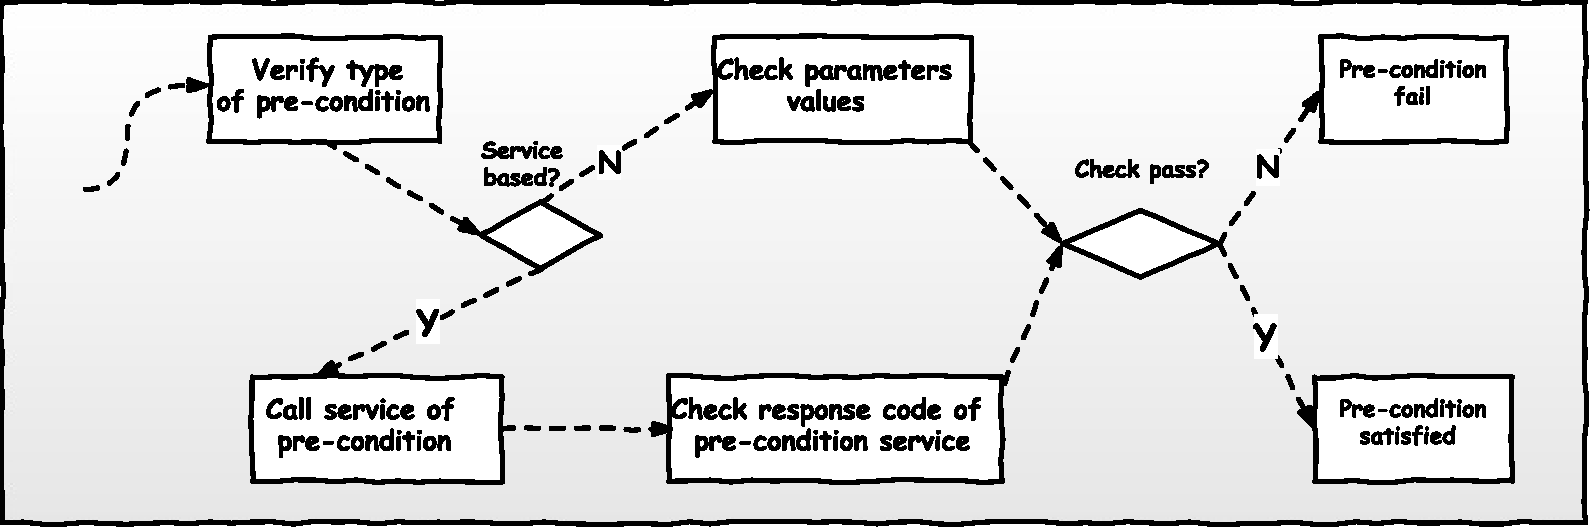
\includegraphics[width=140mm,trim = 0mm 0mm 0mm
0mm,clip]{img/FluxoPrecondicoes.pdf}
\caption{Diagrama de atividades do processamento da precondição}
\label{FigServicePrecondition}
\end{figure}


\subsection{Verificação das pós-condições}
\vspace{-6mm}

\begin{figure}[!htb]
\centering
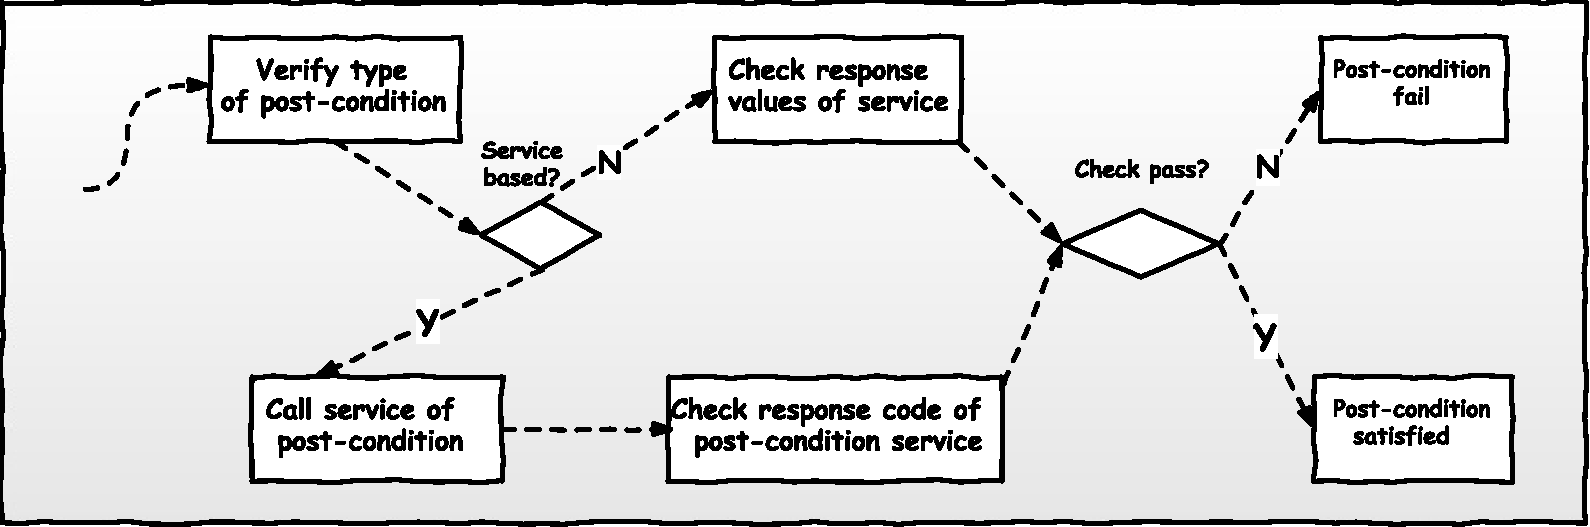
\includegraphics[width=140mm,trim = 0mm 0mm 0mm
0mm,clip]{img/FluxoPostcondicoes.pdf}
\vspace{-6mm}
\caption{Diagrama de atividades do processamento da pós-condição}
\label{FigServicePostcondition}
\end{figure}

A verificação das pós-condições acontece de modo muito similar a das
precondições. Há também os dois tipos, baseado em valores e em chamadas a
outros serviços. O diferencial está em que a validação dos valores passa a
ocorrer a partir dos valores contidos na mensagem de retorno. A Figura
\ref{FigServicePostcondition} descreve as etapas necessárias para validação de
cada precondição.


\section{EXTENSÃO DA NEOIDL PARA DESIGN-BY-CONTRACT}
\label{extensaoNeoIDL-DbC}

A sintaxe escolhida para possibilitar a especificação de pré e pós condições
na \neoidl{} foi influenciada por três linguagens e extensões de linguagens de
programação: Eiffel, JML e Spec\# (exemplificadas na subseção
\ref{implementDbC}). 

Em Eiffel, as asserções são expressões booleanas, de modo que uma pré e uma
poscondição podem ter resultado verdadeiro ou falso. As asserções também podem
incluir chamadas a funções, extendendo a validações a lógicas mais sofisticadas
\cite{meyer1992applying}. Essas caracteríticas, por serem simples e versáteis,
foram consideradas adequadas e incorporadas à especificação de
\designbycontract{} em contratos de serviços na \neoidl{}.

A primeira sintaxe de \designbycontract{} na \neoidl{} teve como
base a sintaxe da JML, especialmente em como se associar as pré e poscondições a
cada serviço ou capacidade, assemelhando-se a comentários e iniciados pelo
símbolo de arroba (@). A figura \ref{lst:precondicaoJML-neo} apresenta um
exemplo de especificação de precondição seguindo a linha da JML.

\vspace{6mm}

\begin{figure}[h]
\begin{small}
\lstinputlisting[language=NeoIDL,firstnumber=1]{trechos_codigo/DBCsimple.neo}
\vspace{-.5cm}
\end{small} 
\caption{Forma preliminar de precondição na \neoidl}
\label{lst:precondicaoJML-neo}
\end{figure}

Essa forma foi apresentada no Workshop de Teses e Dissertações do CBSoft em 2015
\cite{lima2015contratos}, ainda nos primeiros estágios do trabalho. Os revisores
apontaram dificuldade de distinguir, na especificação, entre as pré e
poscondições e as capacidades, pois possuiam prefixos muito
semelhantes (ver linhas 6 a 8).
Essas críticas impulsionaram a busca por outra sintaxe mais adequada aos elementos textuais já
existentes na \neoidl{}.

Spec\# possui uma forma de especificação de asserções em que as pré e
poscondições são declaradas logo após a assinatura do método ou classe, apenas
com o uso das palavras reservadas \emph{require} e \emph{ensure}, sem uso de
símbolos. Essa abordagem foi aplicada à \neoidl{} para versão final da sintaxe
com suporte a \designbycontract{}.

As próximas subseções apresentam alguns exemplos de especificação de pre e
poscondições na \neoidl{} e as mudanças introduzidas na sintaxe da linguagem.
Inicialmente as condições de \designbycontract{} são demonstradas separadamente
e, ao final, a subseção \ref{SintaxeGeralDbc} consolida o conjunto
de novos elementos sintáticos e como eles são estruturados.


\subsection{Precondição básica}
\label{precondicaoBasica}

Uma precondição básica é a que valida os valores recebidos na
requisição, comparando-os com os valores estabelecidos na instrução
\emph{require} do contrato. Esse tipo de precondição assemelha-se a validação
dos atributos recebidos por um método no paradigma de orientação a objetos.

A origem das informações, isto é, onde os valores que serão validados se
encontram, depende da operação HTTP utilizada. A subseção \ref{FonteDadosDbc} descreve como esses
dados são obtidos. Para realizar a comparação do valor recebido com o valor
esperado, a \neoidl{} admite seis operadores de comparação (Subseção
\ref{TiposContrDbC}).

A Figura \ref{lst:DBCPreCondBasica} (linhas 7 e 8) apresenta um exemplo de
precondição básica em uma forma simples, em que apenas um valor é testado (id)
e, caso a condição não seja satisfeita, a instrução \emph{otherwise} indica o
valor a ser retornado (código HTTP Not Found). 	

\begin{figure}[htb]
\begin{small}
\lstinputlisting[language=NeoIDL,firstnumber=1]{trechos_codigo/store_pre_basica.neo}
\end{small}
\caption{Exemplo de notação de precondição básica na \neoidl{}}
\label{lst:DBCPreCondBasica}
\end{figure} 



\subsection{Pós-condição básica}

Em termos sintáticos, as pós-condições básicas possuem uma forma muito
semelhante às precondições básicas (\ref{precondicaoBasica}), diferindo-se
exclusivamente pelo uso da instrução \emph{ensure}. A Figura
\ref{lst:DBCPosCondBasica} (linhas 8 e 9) mostra um exemplo de pós-condição
básica em que, após a execução da operação \method{GET}, se o valor do atributo
\emph{quantity} não for maior que zero, então o serviço não foi executado adequadamente e a exceção
(\emph{otherwise}) é retornada.

\begin{figure}[htb]
\begin{small}
\lstinputlisting[language=NeoIDL,firstnumber=1]{trechos_codigo/store_pos_basica.neo}
\end{small}
\caption{Exemplo de notação de pós-condição básica na \neoidl{}}
\label{lst:DBCPosCondBasica}
\end{figure} 


\subsection{Precondição com chamada a serviço}

As precondições baseadas em serviços seguem uma sequência que envolve a chamada
a outro serviço antes do processamento do serviço principal, em um tipo simples de
composição de serviço. Essa abordagem permite que precondições complexas sejam
validadas por serviços especializados, sem que a especificação do contrato
de serviço seja complexa. Essa proposta preserva ainda a ideia original de
Eiffel\cite{meyer1988eiffel}, de que pré e pós-condições sejam expressões
\emph{booleanas}.

A primeira etapa do processo de execução da precondição de serviço consiste em
fazer a chamada a um serviço (ver Figura \ref{FigServicePrecondition}) por meio de uma
operação \method{GET}. Em seguida, o código de \textit{status} retornado pelo
serviço da precondição é comparado com o valor especificado na precondição do contrato.

Após o acionamento do serviço da precondição, o comportamento é mesmo da
precondição básica (ver \ref{precondicaoBasica}). Caso a precondição seja
satisfeita, é retornado o valor indicado pela instrução \emph{otherwise}. As
precondições de serviço na \neoidl{} admitem os mesmos operadores de comparação
que as precondições básicas.

A Figura \ref{lst:DBCPreCondServico} ilustra a especificação de uma precondição
do tipo serviço (linhas 8 e 9). Assim, antes de executar a operação \method{POST}
do serviço principal, o serviço \emph{store.getOrder} é acionado. Caso esse
serviço retorno o código correspondente a \emph{HTTP Not Found}, a operação
\method{POST} é executada. Caso contrário, o serviço principal retorna o valor
correspondente a \emph{HTTP Invalid Precondition}, em razão do estabelecido no
\emph{otherwise}.


\begin{figure}[htb]
\begin{small}
\lstinputlisting[language=NeoIDL,firstnumber=1]{trechos_codigo/store_pre_servico.neo}
\end{small}
\caption{Exemplo de notação de precondição com chamada a serviço na
\neoidl{}} 
\label{lst:DBCPreCondServico}
\end{figure} 



\subsection{Pós-condição com chamada a serviço}
\label{Pos-condicao servico}

A pós-condição com chamada a serviço seguem a sequência de eventos indicada na
Figura \ref{FigServicePostcondition}. No caso da pós-condição, a execução do
serviço principal já ocoreu e a função do serviço na pós-condição é validar se a
execução do serviço principal ocorreu com sucesso. Algumas pós-condições são
naturais, como as que verificam se um objeto foi inserido após a operação de
inclusão (método \method{POST}). Ou ainda, a que verifica se o objeto foi excluído
após uma operação \method{DELETE}.

No exemplo da Figura \ref{lst:DBCPosCondServico}, o serviço principal faz a
exclusão de um objeto \textit{Order}. A pós-condição (linha 8) verifica, após o
processamento do \method{DELETE}, se o objeto foi efetivamente apagado por meio do
serviço \emph{store.getOrder}. Se o serviço da pós-condição retornar o valor
\emph{HTTP Not Found}, o objeto foi adequadamente excluído. Caso contrário, o
serviço principal retornará o valor \emph{HTTP Not Modified}, o qual foi
estabelecido na instrução \textit{otherwise}.

\begin{figure}[htb]
\begin{small}
\lstinputlisting[language=NeoIDL,firstnumber=1]{trechos_codigo/store_pos_servico.neo}
\end{small}
\caption{Exemplo de notação de pós-condição com chamada a serviço na
\neoidl{}}
\label{lst:DBCPosCondServico}
\end{figure} 


\subsection{Sintaxe geral de pré e pós-condições}
\label{SintaxeGeralDbc}

Entre as subseções \ref{precondicaoBasica} e \ref{Pos-condicao servico} foram
apresentados separadametne exemplos simples de especificação de pre e condições
na \neoidl{} de modo a facilitar a compreensão. Esta subseção demonstra
a estruturação sintática das construções de \designbycontract{} agregadas
\neoidl{} por este trabalho.

\subsubsection{Listas de pré e pós-condições}

Um módulo \neoidl{} possui uma seção para declaração dos serviços (ver Figura
\ref{fig:moduloNeoIDL}). Cada serviço declarado na \neoidl{} pode ter um mais
capacidades, as quais correspondem às operações HTTP utilizadas na arquitetura
REST. Sintaticamente, um serviço possui uma lista de capacidades\footnote{Os
símbolos ``[`` e ``]'' identificam uma lista.}:

\begin{center}
\hilight{\{\texttt{Serviço [Capacidade]}\}}
\end{center}

A sintaxe da \neoidl{} foi extendida para admitir a vinculação de pré e
pós-condições às capacidades. Essas contruções de \designbycontract{} são
opcionais, ou seja, uma capacidade pode não ter nenhuma pré ou pós-condição. Por
outro lado, pode-se incluir nas capacidades mais de uma precondição e mais de
uma pós-condição ou ainda qualquer combinação delas, simultâneamente.

\begin{center}
\hilight{\{\texttt{Capacidade \textcolor{red}{[Condição DbC]}}\}}
\end{center}

É possível ainda, caso uma precondição ou pós-condição se aplique a todas as
capacidades de um serviço, é possível declará-la para o serviço como um todo,
logo antes da declaração das capacidades:

\begin{center}
\hilight{\{\texttt{Serviço \textcolor{red}{[Condição DbC]} [Capacidade]}\}}
\end{center}

 Assim, generalizando, a \neoidl{} passou a suportar a seguinte sintaxe:
 
\begin{center}
\hilight{\{\texttt{Serviço \textcolor{red}{[Condição DbC]} [Capacidade
\textcolor{red}{[Condição DbC]} ]}\}}
\end{center}
 

\subsubsection{Tipos de construções de \designbycontract{}}
\label{TiposContrDbC}

Conforme exemplificado entre as subseções \ref{precondicaoBasica} e
\ref{Pos-condicao servico}, as construções de \designbycontract{} possuem as
seguintes estruturas:

\begin{center}
\hilight{Condição básica: \textbf{TipoCondição} \{\texttt{[Argumento Comparação
Valor]}\}}
\hilight{Condição serviço: \textbf{TipoCondição} \{\texttt{Serviço (Parâmetro)
Comparação ValorSrv}\}}
\hilight{Exceção: \textbf{Otherwise} \{\texttt{Valor de Retorno	}\}}

\end{center}

Onde:
\vspace{-6mm}
\begin{description}
\item [TipoCondição] indica se é uma precondição (\emph{require}) ou uma
pós-condição (\emph{ensure});

\item [Argumento] indica o nome do atributo que será testado;

\item [Comparação] indica o operação de comparação que a ser utilizada. A
\neoidl{}  admite seis operadores de comparação: igualdade (\literal{==}), 
diferença (\literal{<>}), maior (\literal{>}), maior ou igual (\literal{>=}), 
menor (\literal{<}) e menor ou igual (\literal{<=}). Eles podem ser aplicados  a
qualquer tipo de pré ou poscondição.

Mais de um atributo pode ser testado em uma pré ou pós-condição. Na expressão
acima, essa característica é simbolizada com a indicação de uma lista.

\item [Valor] corresponde ao valor que será comparado com o \textbf{Argumento}.
As pré e pós-condições básicas admitem algumas combinações com os operadores
\emph{not}, \emph{and} e \emph{or}, formando expressões booleanas e,
assim, permitindo estabelecer regras mais abrangentes.

Por exemplo, a precondição apresentada na Figura \ref{lst:DBCPreCondBasica} poderia
ser escrita como \emph{\textbf{require} (\textbf{not} id \literal{<=} 0)}. Os
operadores \emph{and} e \emph{or} são infixos (ex.: \emph{\textbf{require}
((id \literal{>} 0 \textbf{or} id \literal{<=} -1000))}). O uso do operador
\emph{and} produz o mesmo efeito de se declarar duas precondições.

\item [Serviço] indica o nome do serviço que será acionado. As informações para
indicação concreta da localização do serviço, ou seja, a URL de acionamento, não
são indicados nesse atributo de pre e pós-condição. Essas informações dependem
do local de implantação do serviço e não convém que estejam declaradas no
contrato, sob pena de que mudanças no ambiente de implantação do serviço gerem
impacto ao contrato.
Entretanto, caso se queira fazer essa vinculação, pode ser criada uma anotação
\neoidl{}, com essa finalidade, para o serviço.

\item [Parâmetro] tem a função de indicar os valores que serão passados para a
chamada ao serviço da pré ou pós-condição.

 \item [ValorSrv] corresponde a um valor que será comparado com o
 \textit{Status Code HTTP} retornado pelo serviço. Na \neoidl{}, esses valores
 são convencionados como o nome do corresponde ao código HTTP, com palavras
 justapostas (Ex.: "NotFound" tem o valor do código 404, de HTTP \textit{Not
 Found})

\item [Valor de Retorno] é utilizado na cláusula \emph{otherwise} para indicar o
valor que o serviço principal deve retornar caso uma precondiçaõ ou pós-condição
não seja atendida.

\end{description}


\subsubsection{Um último exemplo de módulo com \designbycontract{}}

A Figura \ref{lst:ModuloNeoVariosDbC} apresenta um exemplo módulo \neoidl{} de
um serviço completo, utilizando alguns dos recursos apresentados na subseção
\ref{TiposContrDbC}. Esse serviço possui três operações, cada uma com duas
condições de \designbycontract{}.

A operação \method{GET} possui uma precondição em que o valor do atributo \emph{id} deve ser maior que zero (linha 8), caso contrário a operação deve retornar o valor
correspondente a "NotFound". Uma pós-condição assegura que, se o serviço for
executado adequadamente, o valor de \emph{quantity} será maior que zero (linha
9). Se for violada a pós-condição, a operação \method{GET} retorna o valor
"NoContent".

A operação \method{POST} possui duas precondições (linhas 13 e 14). A primeira,
básica, valida o valor do atributo \emph{quantity}. A segunda, aciona o serviço
\emph{store.getOrder} com o parâmetro \emph{id}. Nessa operação, foi
definido um valor de exceção único para as duas precondições. A \neoidl{}
associa essa instrução de \emph{otherwise} geral às instruções anteriores que
não possuem condição e exceção específica (caso da linha 8).

Na operação \method{DELETE} foi utilizado o operador lógico \emph{and} na
precondição (linha 18). A pós-condição faz a chamada ao serviço
\emph{store.getOrder}. Tanto a pré como a pós-condição possuem o mesmo valor de
exceção (linha 20). 

\begin{figure}[htb]
\begin{small}
\lstinputlisting[language=NeoIDL,firstnumber=1]{trechos_codigo/store_dbc_complete.neo}
\end{small}
\caption{Exemplo de módulo \neoidl{} com várias instruções de \designbycontract{}}
\label{lst:ModuloNeoVariosDbC}
\end{figure} 	



\subsection{Fontes de dados para pré e pós-condições}
\label{FonteDadosDbc}

Os serviços REST na \neoidl{} seguem uma convenção em relação ao conteúdo
presente na requisição e na resposta para cada tipo de operação \emph{HTTP},
conforme descrito na subseção \ref{linguagemNeoIDL}. Por exemplo, o método \method{GET}
submete os argumentos pelo \emph{path} ou como \textit{query string} da
requisição e não em seu corpo. Esses aspectos foram considerados para se definir
a fonte das informações para os argumentos e parâmetros utilizados nas pré e
pós-condições.

A Figura \ref{Fig:FonteDadosDbcNeoIDL} resume a origem para cada operação. Há
diferenças também entre os tipos básico e baseado em serviços das construções de
\designbycontract{}. As operações \method{GET} e \method{DELETE} não possuem
argumentos encaminhados no corpo da requisição. Para essas operações, os
argumentos são retirados do \emph{path} ou \emph{query string} para validação
das precondições, tanto no tipo básico como no tipo baseado em composição. Na
figura, essa origem é identificada como \textit{Request arguments}.

\begin{figure}[!htb]
\centering
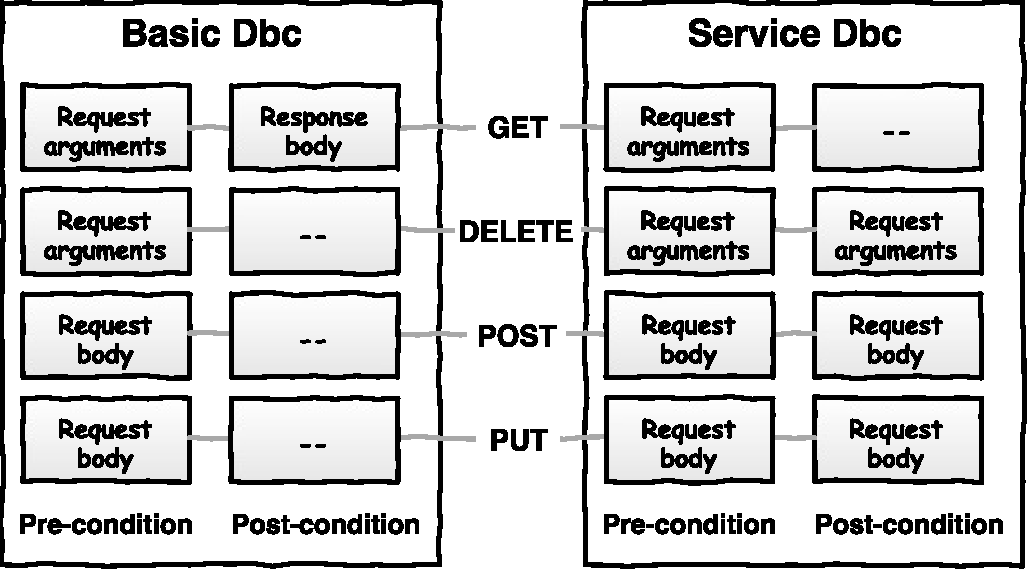
\includegraphics[width=120mm,trim = 0mm 0mm 0mm
0mm,clip]{img/FonteDadosDbcNeoIDLIngles.pdf}
\caption{Diagrama da fonte de dados para acionamento de pré e pós-condições}
\label{Fig:FonteDadosDbcNeoIDL}
\end{figure}


Por outro lado, as operações \method{POST} e \method{PUT} submetem os dados a
serem inseridos ou alterados pelo corpo da requisição (\textit{Request body}),
local de onde as precondições básicas e baseadas em serviços devem extrair os
parâmetros de validação.
A \neoidl{} utiliza a notação JSON\cite{JSon} no corpo das requisições. A
representação dos argumentos utiliza o padrão separado por pontos para indicar
elementos mais internos (ex. "Pessoa.Nome").

No caso das pós-condições, a origem das informações diverge entre o tipo
básicos e o tipo por serviços. A única operação que admite pós-condição básica é
a operação \method{GET}, em que os argumentos de validação são extraídos do
corpo da resposta (\textit{Response body}). As demais operações não retornam dados
no corpo da requisição, pois estão voltadas para alteração de informações e não
para consultas. Além disso, não há utilidade em se validar dados de requisição
em uma pós-condição.

Já as pós-condições baseadas em serviços não suportam a operação \method{GET}.
Embora seja tecnicamente possível acionar um serviço com base nos argumentos da
requisição, como não se tem modificação nos dados por essa operação, a
validação dessas informações pode meio de serviço deve ser feita nas
precondições. Ademais, as pós-condições básicas da operação \method{GET} cumprem
com o objetivo que validar as informações de saída.

A pós-condição da operação \method{DELETE} pode acionar serviços com base nos
argumentos da requisição (\textit{Request arguments}). Um caso típico é de
acionar o serviço de consulta para verificar se o dado foi efetivamente
excluído. As operações \method{POST} e \method{PUT} podem acionam serviços em
pós-condições utilizando as informações do corpo da requisição (\textit{Request
body}), uma vez que essas operações não possuem dados no corpo da resposta. 



\section{ESTUDO DE CASO: PLUGIN TWISTED}
\label{pluginTwisted}

A incorporação de regras de \designbycontract{} aos contratos para
serviços REST escritos em \neoidl{} elevam a um novo patamar os níveis de
garantias com a estabilidade comportamental dos serviços. Nesse sentido, a
preocupação em garantir ao cliente que o serviço proverá as informações de que
ele necessita aumenta, reforçando os benefícios observados com a prática
\CtFirst{}. Ou seja, o desenho do serviço considera ainda mais a perspectiva do
consumidor do serviço.

A seção \ref{extensaoNeoIDL-DbC} tratou do elemento \emph{Contrato}, sobre como
ele pode ser escrito em \neoidl{} com suporte a construções de
\designbycontract{}. O contrato, porém, é apenas uma especificação, no
sentido de descrever regras e não de torná-las executáveis em si. Todavia, a
\neoidl{} é, além de uma linguagem formal, um \framework{} de geração de
código poliglota (subseção \ref{histMotivNeoIDL}) por meio de plugins.

Para se comprovar a viabilidade de se conceber serviços com suporte a pré e
pós-condições, foi desenvolvido, no decorrer da pesquisa de mestrado, um plugin
da \neoidl{} que cumpre com tal finalidade. As próximas subseções detalham como
é estruturada a arquitetura do serviço gerado e seu comportamento em relação a
\designbycontract{}. Ao final, alguns aspectos sobre a implementação do
próprio plugin são descritos.

\subsection{Visão geral do Python \twisted{}}
\label{PythonTwisted}

Adotou-se o \framework{} \emph{Python Twisted}\cite{fettig2005twisted} como tecnologia para
construção dos serviços com pré e pós-condições. A escolha se deu em razão de
\twisted{} possuir uma arquitetura voltada para processamento de requisições de vários
tipos de protocolos de rede sobre uma infraestrutura simples e autônoma. 

O \twisted{} é baseado em eventos e adota a estratégia de tratamentos de
requisições de forma assíncrona, em detrimento ao uso de \textit{threads}. O
núcleo do \twisted{} é o \textit{loop} do objeto \emph{reactor} responsável por
aguardar e direcionar o processamento dos eventos (Figura
\ref{Fig:TwistedReactor}). Uma requisição HTTP, como as das chamadas a serviços REST, são tratados como
eventos.

\begin{figure}[!htb]
\centering
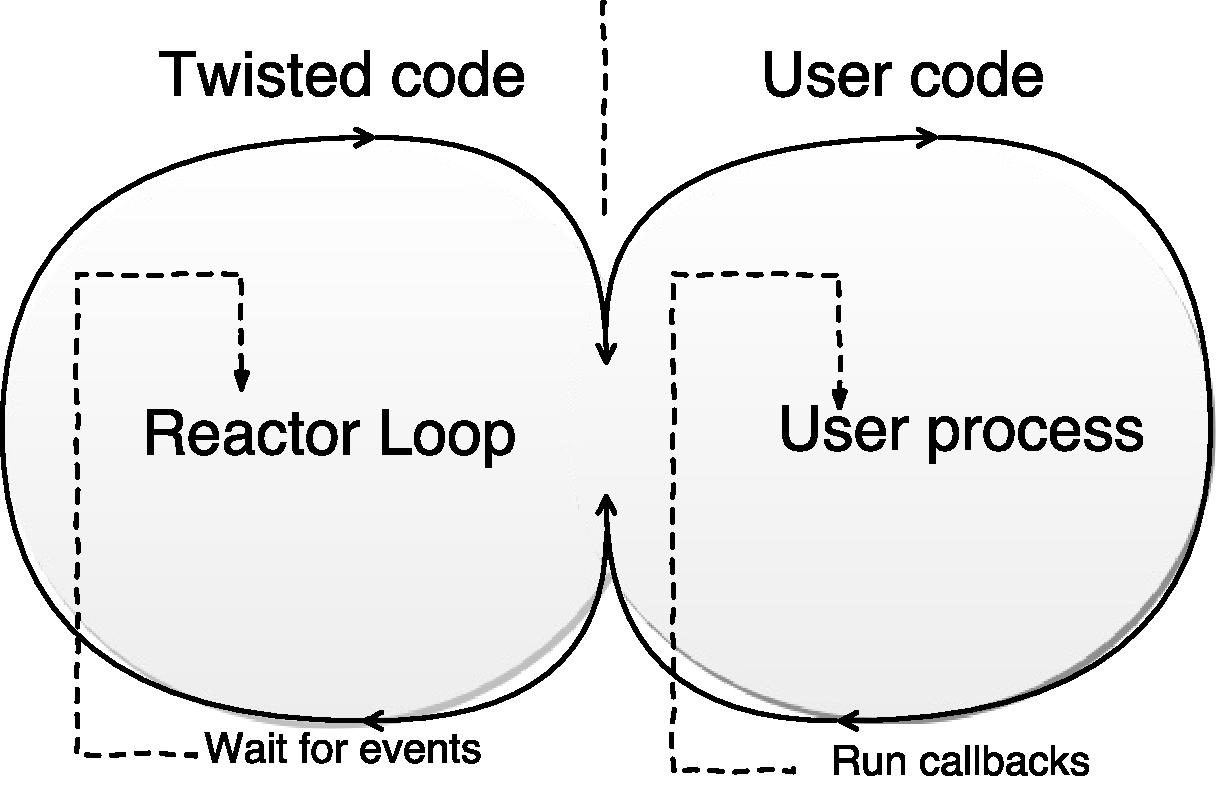
\includegraphics[width=80mm,trim = 0mm 0mm 0mm
0mm,clip]{img/TwistedReactor.pdf}
\caption{Arquitetura assíncrona do \twisted{}}
\label{Fig:TwistedReactor}
\end{figure}

O \emph{reactor} entrega os eventos para serem tratados para processamentos
especializados, indicados no lado direito da Figura \ref{Fig:TwistedReactor}.
Caso o processamento de um evento seja lento, deve-se disparar um
processamento assíncrono, e registrar no \emph{reactor} uma chamada para quando
o processamento assíncrono se encerrar, o qual será tratado como um outro
evento.
Esse controle é feito por um objeto denominado \emph{Deferred}, que contém uma lista
de \emph{Callbacks} \cite{fettig2005twisted}.


\subsection{Arquitetura dos serviços \twisted{}}
\label{ArquiteturaTwisted}

Os serviços \twisted{} gerados pela \neoidl{} são estruturados em uma
arquitetura que extende a arquitetura base do \twisted{} \emph{Reactor},
incorporando serviços ao processamento das requisições, como ilustrado na Figura
\ref{Fig:TwistedReactorServices}. Os serviços são autônomos entre si, e
processam as requisições de acordo com o roteamento realizado pelo servidor.

\begin{figure}[!htb]
\centering
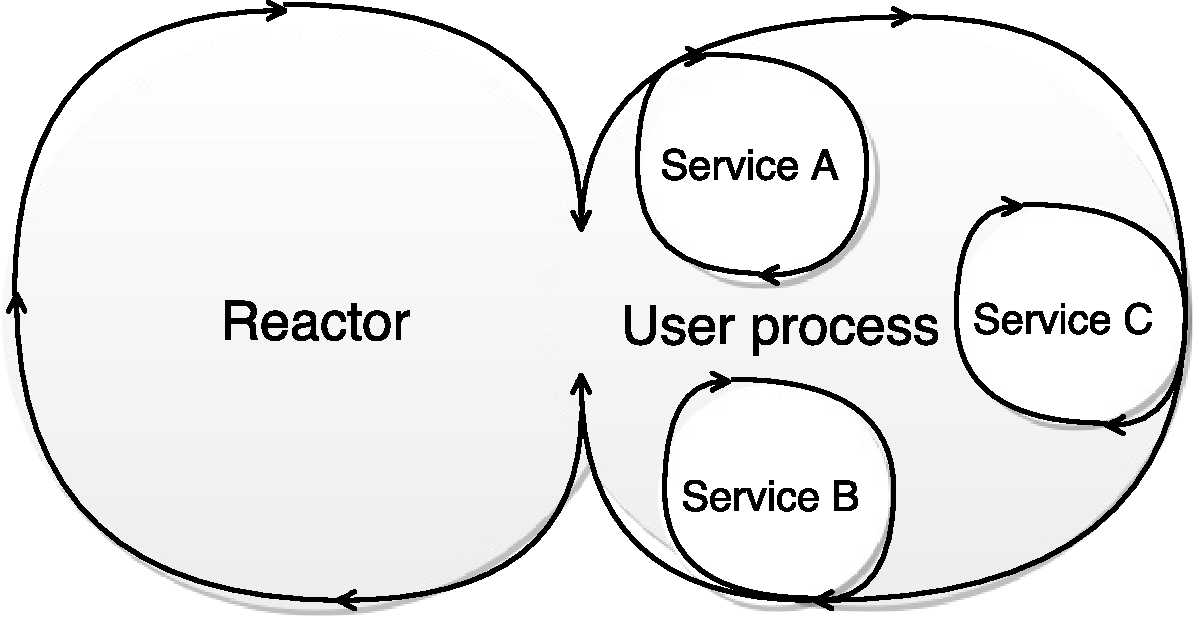
\includegraphics[width=80mm,trim = 0mm 0mm 0mm
0mm,clip]{img/TwistedReactorServices.pdf}
\caption{Operação dos serviços na arquitetura \twisted{}}
\label{Fig:TwistedReactorServices}
\end{figure}

Em termos de classes, a \neoidl{} gera um conjunto de tres módulos base,
que constituem o pacote do \twisted{} \textit{server}, representados na
parte superior da Figura \ref{Fig:TwistedArchtecture}. Essas classes são fixas,
ou seja, não dependem da quantidade nem do conteúdo dos serviços declarados no
módulo \neoidl{}.

A classe \emph{Server} é o núcleo do \twisted{} \textit{server}. Ela é
responsável por subir o servidor HTTP, receber as requisições, identificar
as operações da requisição (\method{GET}, \method{POST}, \method{PUT} ou \method{DELETE}), e
direcionar a requisição para o serviço específico. A identificação do serviço é
feita por meio de um arquivo de rota (routes.json), o qual possui uma tradução
entre os \emph{paths} das requisições e os serviços responsáveis por cada uma
delas.

A classe \emph{Utils} contém um conjunto de funções utilitárias, como a que
realiza o \textit{parse} da requisição para extrair os argumentos repassados
na URI ou \textit{query string}. Ela também define o objeto que trafega a
resposta dos serviços entre os serviço e o servidor.

Essas duas classes são suficientes para o servidor quando não se utiliza
\designbycontract{} nos serviços. O pacote
\emph{DbcConditions} consolida o conjunto de classes responsáveis por processar
as pré e pós-condições. A principal função de \emph{DbcConditions} é realizar a
comparação entre o valor real e o valor esperado, efetivando toda a
lógica corresponde às construções de \designbycontract{} descritas na subseção
\ref{TiposContrDbC}.

\begin{figure}[htb]
\centering
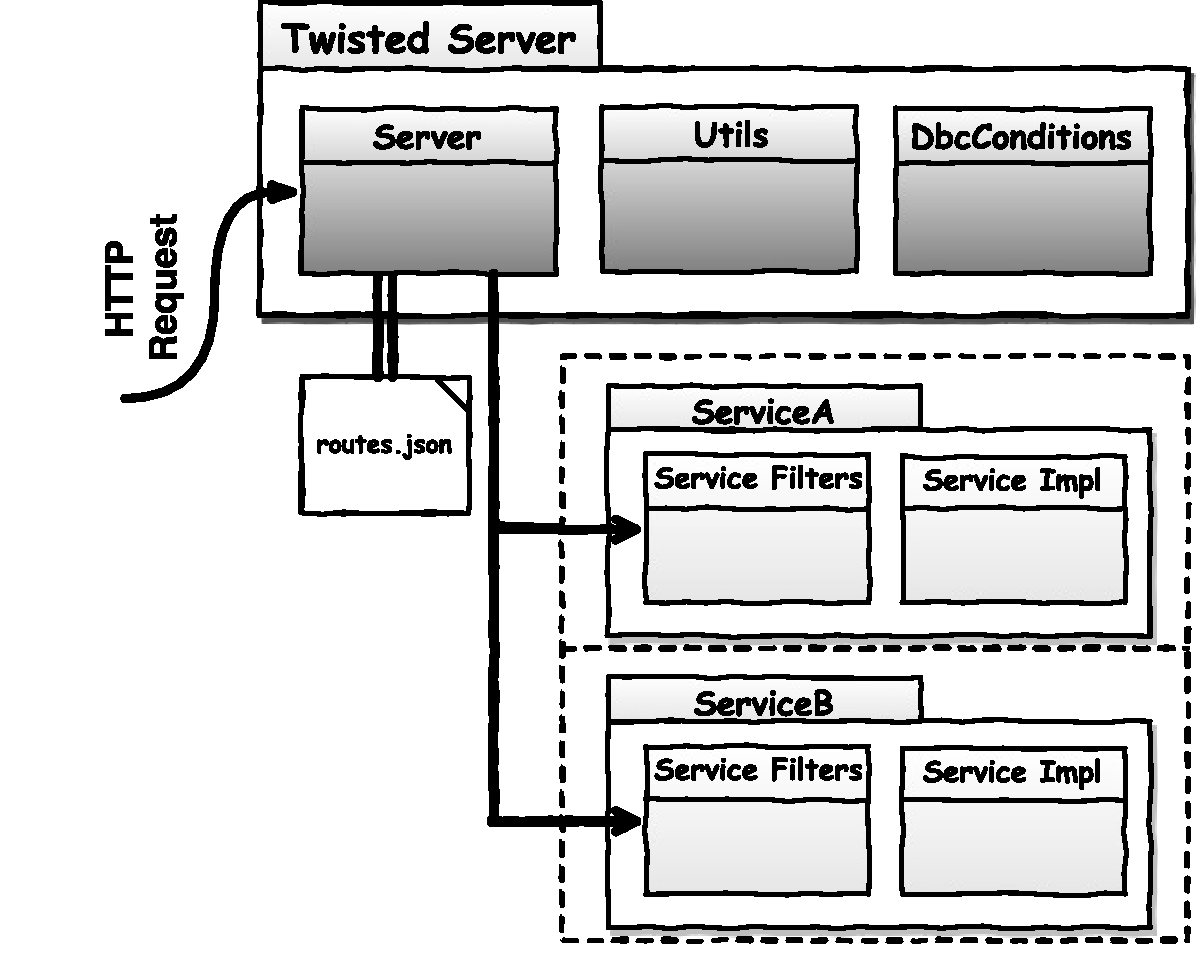
\includegraphics[width=90mm,trim = 18mm 4mm 0mm
0mm,clip]{img/TwistedServer.pdf}
\caption{Arquitetura do serviço Twisted gerado pela \neoidl{}}
\label{Fig:TwistedArchtecture}
\end{figure}

Em \emph{DbcConditions} estão as funções que carregam a lista de pré e
pós-condições para cada serviço. A chamada para as pré e pós-condições baseadas
em serviços também é construída nesse pacote. Essa pacote é fundamental para o
funcionamento das construções de \designbycontract{} e consta transcrita no
Apêndice \ref{classesDbcCondition}.

Para cada serviço declarado no módulo \neoidl{} são geradas duas classes: os
filtros do serviço e o serviço em si. A classe \emph{ServiceFilter} recebe a
requisição; carrega e processa as precondições; aciona o serviço e; ao final,
carrega e processa as pós-condições. Esse modo de operação dos filtros é
ilustrado na Figura \ref{Fig:TwistedFiltes}. A classe do serviço, por
fim, contém apenas a estrutura para implementação da lógica interna do serviço.

\begin{figure}[!htb]
\centering
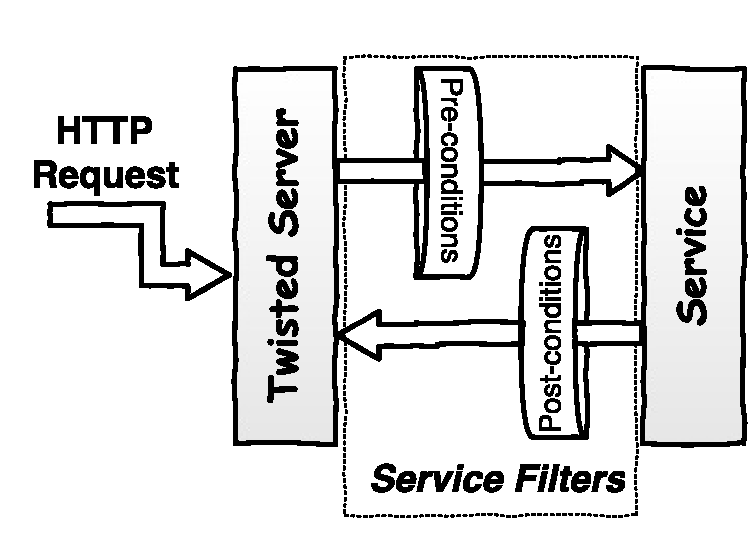
\includegraphics[width=80mm,trim = 5mm 6mm 0mm 
3mm,clip]{img/TwistedFilters.pdf}
\caption{Modo de operação das pré e pós-condições no serviço Twisted}
\label{Fig:TwistedFiltes}
\end{figure}



\subsection{Geração de código}

O plugin \twisted{} é um conjunto de seis módulos Haskell. Para cada tipo de
arquivo gerado, há um módulo no plugin, conforme Figura \ref{PluginTwisted}. Os
módulos \emph{PPService}, \emph{PPUtils} e P\emph{PDbcConditions} apenas
imprimem um código Python fixo, sem qualquer interferência do módulo \neoidl{}
processado. \emph{PPRoute} é um pequeno módulo (42 linhas) que processa as
informações contidas nas instruções \emph{path} dos serviços declarados no
módulo \neoidl{} e mapeia a correspondência entre as URIs e os serviços.

\begin{figure}[!htb]
\centering
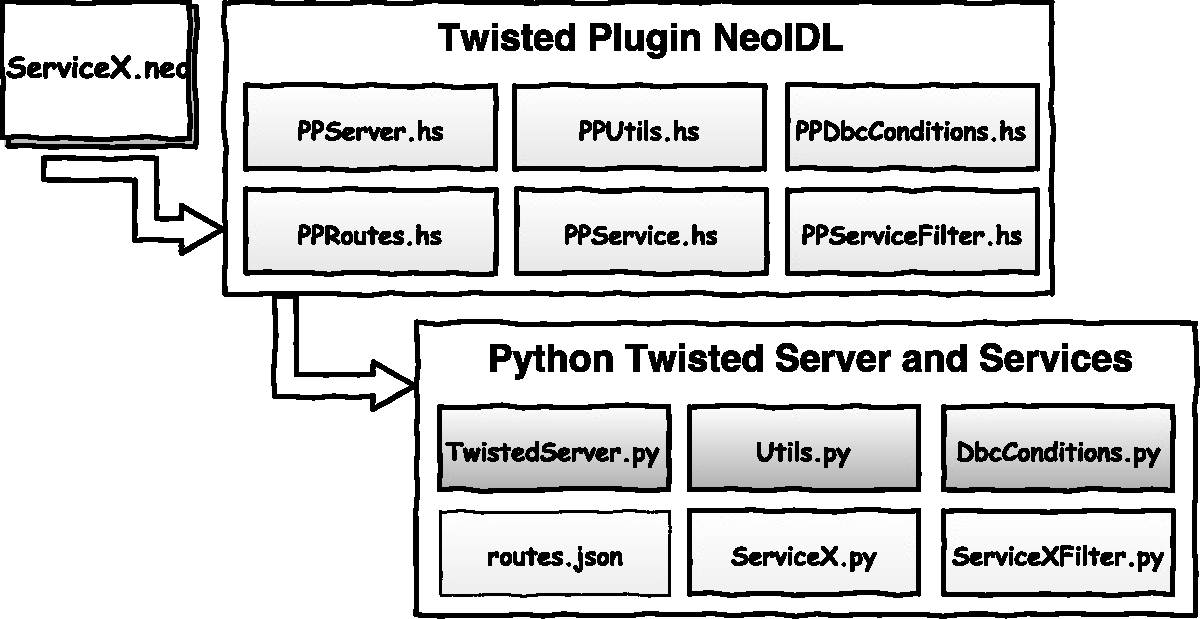
\includegraphics[width=100mm,trim = 0mm 0mm 0mm 
0mm,clip]{img/PluginTwisted.pdf}
\caption{Plugin para geração de código Twisted com suporte a \designbycontract{}}
\label{PluginTwisted}
\end{figure}

O módulo \emph{PPService} gera uma classe com um método para cada operação do
serviço. Na versão atual do plugin, os métodos são implementados com uma lógica
de gravação de objetos em um banco em memória, apenas para simplificar o teste
dos código gerado. Essa implementação não é relevante, uma vez que a lógica
especializada do serviço real a substituirá.

A parte correspondente ao acionamento das pré e pós-condições é produzido pelo
módulo \emph{PPServiceFilter}. O código produzido por este módulo é composto de
duas seções: (i) a declaração das condições de \designbycontract{} e (ii) o
carregamento dessas condições. A primeira seção, de declaração das condições
\designbycontract{} contém a lista de pré e pos-condições do serviço. A Figura 
\ref{Fig:LhsRhsDbcConditions} apresenta um exemplo de condição especificada em
\neoidl{} transformada em código \emph{Python Twisted}.

O lado esquerda dessa
figura contém a especificação de uma pós-condição (\emph{\textbf{ensure}}, na
linha 2) associada à operação \method{GET} (linha 1). Constitui-se de uma
pós-condição básica, que testa se o valor de resposta \emph{quantity} é maior que zero
(linhas 3 a 5). Caso a pós-condição não seja satisfeita, o serviço retorna o
código \emph{HTTP No Content}.


\setbox0=\hbox{%
%\begin{minipage}{1.9in}
\begin{minipage}{6cm}
\begin{lstlisting}[
basicstyle={\tiny\ttfamily},
identifierstyle={\color{black}},
tabsize=2,
language={NeoIDL},
numbersep=8pt,
numbers=left,
xleftmargin=0.5cm,frame=tlbr,framesep=2pt,framerule=0pt,
morekeywords ={class,run}
]
@get    Order getOrder (int id)
		ensure (
				quantity
				>
				"0"
		),
		otherwise "NoContent";
\end{lstlisting}
\end{minipage}
}
\savestack{\listingA}{\box0}

\setbox0=\hbox{%
\begin{minipage}{6cm}
\begin{lstlisting}[
basicstyle={\tiny\ttfamily},
identifierstyle={\color{black}},
tabsize=2,
language={PythonTwisted},
numbersep=8pt,
numbers=left,
xleftmargin=0.5cm,frame=tlbr,framesep=2pt,framerule=0pt,
morekeywords ={class,run}
]
self.list.append(
	DbcCheckBasic(
		'quantity',
		'>',
		'0',
		204,
		ValuesSource.responseBody,
		DbcConditionType.PostCondition,
		OperationType.GET
	)
)
\end{lstlisting}
\end{minipage}
}
\savestack{\listingB}{\box0}

\begin{figure}[h]
\begin{center}
\begin{tabular}{|c|c|c|}
\hline
%\stackinset{l}{-5pt}{t}{13\llength}{$\bullet$}{\listingA} &
%\stackinset{l}{-5pt}{t}{ 7\llength}{$\bullet$}{\listingB} \\
\stackinset{l}{-5pt}{t}{}{}{\listingA} &
 &
\stackinset{l}{-5pt}{t}{}{}{\listingB} \\
\hline
\end{tabular}

\caption{Transformação de pós-condição \neoidl{} (lado esquerdo) em código
Python \twisted{} (lado direito)}
\label{Fig:LhsRhsDbcConditions}
\end{center}
\end{figure}

Do lado direito da Figura \ref{Fig:LhsRhsDbcConditions} está o código
\emph{Python Twisted} correspondente. O motor de transformação identifica que a
condição especificada é uma pós-condição básica (classe \emph{DbcCheckBasic} na linha 2
e tipo na linha 8) associada uma operação \method{GET} (linha 9). Conforme
convenção adotada sobre a fonte de informações (Subseção \ref{FonteDadosDbc}), a
pós-condição é carregada com a indicação de que os argumentos devem ser lidos do
corpo da resposta do serviço (linha 7).

Os parâmetros da pós-condição possuem uma correspondência direta, em que as
linhas 3 a 5 do lado esquerdo correspondem também às linhas 3 a 5 do lado
direito. O valor de exceção da especificação \neoidl{} é traduzido no código
HTTP correspondente (linha 6). Ambos os códigos apresentados na Figura
\ref{Fig:LhsRhsDbcConditions} são, na realidade, escritos em uma única linha.
O uso de múltiplas linhas foi adotado aqui apenas para efeitos didáticos.

A segunda seção da classe \emph{ServiceFilter} é genérica para
qualquer serviço. A Figura \ref{lst:filtrosServicosTwisted} contém um trecho
dessa seção. Cada método se inicia com o carregamento das precondições (linha
10), seguindo pelo acionamento do serviço principal (linha 12). Por fim,
as pós-condições são carregadas (linha 14).

\begin{figure}[h]
\begin{small}
\lstinputlisting[language=PythonTwisted,firstnumber=1]{trechos_codigo/serviceFilterLoad.py}
\vspace{-.5cm}
\end{small} 
\caption{Seção de código do filtro de serviços}
\label{lst:filtrosServicosTwisted} 
\end{figure} 


\section{ESTUDO EMPÍRICO DA ANÁLISE SUBJETIVA} 
\vspace{-6mm}

\ldots

\ldots

\label{analiseSubjetiva}
\vspace{-6mm}

%%%%
A language's expressiveness is the major criterion for choosing a language to
state a given set of facts: a language that cannot express the facts should not
be used. However, additional criteria are needed to choose among languages that
are sufficiently expressive  for a set of facts. Two of these criteria are how
ease it is to state the facts in the language and how easy is to perceive the
facts once they are stated.

expressividade de uma linguagem é o principal critério para a escolha de uma
linguagem para indicar um determinado conjunto de fatos: uma linguagem que não
podem expressar os fatos não devem ser usados. No entanto, os critérios
adicionais são necessários para escolher entre os idiomas que são
suficientemente expressivo para um conjunto de fatos. Dois desses critérios são
quão fácil é expor os fatos na linguagem e como é fácil de perceber os fatos,
uma vez que são demonstrados.

\cite{mackinlay1985expressiveness}

%%%%


%%%
Instead of aiming to be the best for solving any kind of
computing problem, DSLs aim to be particularly good for
solving a specific class of problems, and in doing so they
are often much more accessible to the general public than tra-
ditional programming languages.
\cite{taha2008domain}
%%%% 

%%%%
They offer substantial gains in expressiveness and ease of use compared
with GPLs in their domain of application’. [2] describes the typical costs of a
DSL, noting that a small extra initial investment in a DSL implementation typ-
ically leads to long term savings, in comparison to alternative routes.
\cite{tratt2008evolving}
%%%%

%%%%
A domain specific language (DSL) is a program-
ming language tailored for a particular application do-
main. Characteristic of an effective DSL is the ability
to develop complete application programs for a do-
main quickly and effectively. A DSL is not (neces-
sarily) “general purpose.” Rather, it should capture
precisely the semantics of an application domain, no
more and no less.

There are lots of advantages to using DSLs, start-
ing with the fact that programs are generally easier to
write, reason about, and modify compared to equivalent 
programs written in general purpose languages.
Indeed, these are the same advantages gained from using any high-level
programming language.
\cite{hudak1998modular}
%%%%




\subsection{Método}
\vspace{-6mm}

\subsection{GQM}
\vspace{-6mm}

\subsection{Questionário}
\vspace{-6mm}

\subsection{Análise dos Resultados}
\vspace{-6mm}


* Questionário montado para avaliar a utilidade de DbC com NeoIDL

* Inicialmente motivado pelo estudo do Alessandro Garcia

* GQM e Avaliação TAM

* Montagem do questionário

1. Perfil técnico-profissional do respondente
1.1 Para qual órgão ou empresa você presta serviços atualmente?
1.2 A quanto tempo você trabalha com desenvolvimento Web
1.3 A quanto tempo você desenvolve com uso de APIs Web (Web Service)
1.4 Qual o seu nível de experiência com especificação de API REST
1.5 Qual o seu nível de experiência com especificação de contratos com Swagger

3 Questões sobre especificação e implementação de APIs Web
3.1 A especificação do contrato formalmente, seja em Swagger ou NeoIDL, em
relação a descrição textual, aumentará meu nível de acerto na implementação (efetividade).
3.2 Identificar e compreender as operações e atributos na especificação Swagger
é simples para mim.
3.3 Identificar e compreender as operações e atributos na especificação NeoIDL é
simples para mim.

4. DbC
4.1 Conhecer previamente e explicitamente as precondições será útil para mim.
(Useful)
4.2 Aprender a identificar as precondições na NeoIDL parece ser simples pra mim
(Easy to learn)
4.3 Parece ser fácil para mim declarar uma precondição na NeoIDL
(Clear and understandable)
4.4 Me lembrar da sintaxe da precondição na NeoIDL é fácil  (Remember)

5. Geração de código
5.1 É claro e compreensível para mim o efeito da precondição sobre o código
gerado  (Controllable)
5.2 A geração do código de pré e pós-condições aumentará minha produtividade na
implementação do serviço (Job performance)
5.3 Assumindo ter a disposição a NeoIDL no meu trabalho, para especificação de
contratos e geração de código, eu presumo que a utilizarei regularmente no futuro.
5.4 Nesse mesmo contexto, eu vou preferir utilizar contratos escritos em NeoIDL
do que descritos de outra forma



* Distribuição do questionário

% \subsubsection{Avaliação dos resultados}
% 
% \begin{figure*}[h]
% \begin{center}
% 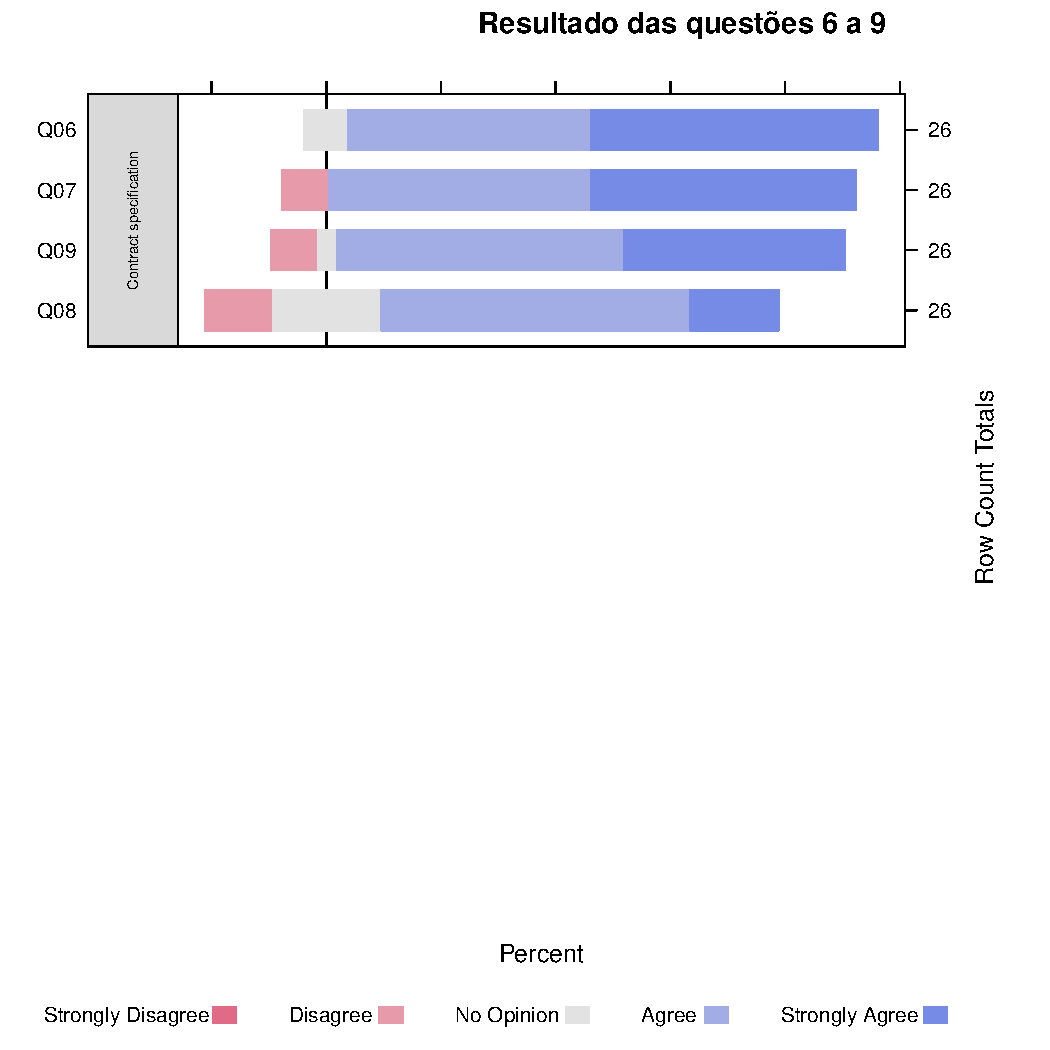
\includegraphics[scale=0.55,trim=0cm 1.5cm 0cm
% 0cm]{img/ResultQuestions06a09.pdf}  
% \end{center}
% \caption{Módulo \neoidl{}}
% \label{fig:moduloNeoIDL}
% \end{figure*}

* Ameaças
- não foi fornecido nenhum material sobre a NeoIDL, apresentando somente o uma
descrição de serviço
- O questionário foi aplicado uma única vez, sem melhorias a partir do primeiro
conjunto de respostas




* Questionários futuros

A principal questão de pesquisa a ser avaliada com o uso do questionário é a utilidade em se agregar ao design das especificações de serviços REST as garantias de pré e
pós-condições. Em segundo momento, pressupondo a utilidade, avaliar se a NeoIDL
cumpre satisfatoriamente com este propósito, agregando à sintaxe da linguagem
a possibilidade de se expressar pré e pós-condições.

* Separar os respondentes em faixas de experiência. Verificar se as respostas
dos menos experientes precisam ser descartadas pela pouca capacidade crítica.
Separar a análise entre os respondentes que conhecem e os que não conhecem
Swagger.

* Perspectivas de comparação
a) Experiência com desenvolvimento com uso de REST
b) Experiência com Swagger
c) Utilidade da especificação formal de contratos
d) Percepção da NeoIDL sem DbC





